\chapter{Conceptual Clusterings, Similarity, and Relatedness} \label{chap:literal}
In Chapter~\ref{chap:theory}, I laid out the theoretical groundwork for statistical context sensitive models of lexical semantics, and in Chapter~\ref{chap:method} I described the actual methodology for building such much.  In this chapter, I will now present the first set of experiments designed to evaluate the utility of this methodology.  These experiments are intended to probe the productivity of a context sensitive, geometric approach to building a computational model of semantics based on statistics about word co-occurrences.  They encompass two different experimental set-ups and corresponding varieties of data, one of which has been designed specifically for the purpose of testing my ideas and one of which involves an assortment of data used pervasively by computational linguistics interested in semantic models.

The first experiment, presented as a proof of concept, involves using multi-word phrases as input and evaluating the methodology's capacity for building subspaces where words associated with the conceptual category denoted by the input term can be reliably discovered.  This experiment expands upon the notion of proto-conceptual spaces outlined in the previous chapter, considering whether the word vectors that populate regions of subspaces are characterised by a certain categorical coherence.  In the case of the data explored here, the experiment is specifically set up to feel out the contextual capacity of my methodology and compare it to a standard generic semantic space.  The question asked is whether the shifts from subspace to subspace based on particular input yield productive alterations in the way that words both cluster and emerge from the melange of word-vectors that circulate around my base model.

The second experiment moves into more familiar computational linguistic territory, using some well-travelled datasets to examine the methodology's capacity for identifying two related but distinct semantic phenomena: relatedness and similarity.  Each of these objectives have provided reliable but distinct evaluative criteria for computational models of lexical semantics.  One of the hypotheses I will put forward regarding my methodology is that the geometrically replete subspaces generated by my contextualisation techniques should provide features for the simultaneous representation of related, diverse, and sometimes antagonistic aspects of language.  Experimenting with these established datasets will provide a platform for exploring the ways in which different features of a semantic structure projected into one of my contextualised subspaces shift as the relationships inherent in the generation of the subspace likewise change, and this will in turn lead to some searching questions about the importance of context in the computational modelling of these particular semantic phenomena in the first place.

\section{A Proof of Concept}
In this section, I present the first experiment performed using my contextually dynamic distributional semantic model.  The gist of this experiment is to take a word pair representing a compound noun -- for instance, \emph{body part} -- and see if my methodology can use the word pair to contextually generate a space where other words conceptually related to that compound noun can be found in a systematic way.  This is conceived of as an entailment task, in that I will attempt to find phrases considered to be categorical constituents of the concept represented by the word pair, taking the WordNet lexical taxonomy as a ground truth.  There is a scholastic back story here.

An early version of this experiment was reported in \cite{AgresEA2015}.  That first effort arose out of a question posed by a colleague regarding the feasibility of using a statical NLP technique for generating categorical labels that could be used to evaluate computational creativity in a domain specific way \citep[for a psychological perspective on the difficulty of generating such terms in an objective way using human subjects, see][]{VanDerVeldeEA2015}.  So, for instance, given a creative domain such as \textsc{musical creativity}, could a distributional semantic model generate terms that are reliably relevant to the concept denoted by that phrase, rather than the potentially disparate properties independently associated with \textsc{music} and \textsc{creativity}?  Intuitively there seems to be little reason to hope that the space halfway between these points in a general semantic space would somehow adequately represent the properties of the overall concept.  The early work explored the dimensions contextually selected by analysing the co-occurrence features of word-vectors corresponding to inputs along the lines of the expository results presented anecdotally in Chapter~\ref{chap:method}, but without any rigorous evaluation.

Reviewer responses to a subsequent journal article \citep{McGregorEA2015c}, designed as a more thorough introduction of the methodology, inspired a computationally oriented mode of evaluation.  The experiment that has emerged involves attempting to recapitulate taxonomical conceptual relationships from the WordNet database \citep{Fellbaum1998}.  Wordnet is a lexical taxonomy of \emph{synsets}, basically semantic word senses, arranged into a hierarchy of entailment relationships, with each synset associate with a number of \emph{lemmas}, word types indexed by that synset according to human annotators.  This experiment takes as input instances of synsets labelled by compound noun phrases and seeks to output as many of the lemmas listed associated with synsets that are hyponyms of the input synset.  So, for instance, the synset \text{body part} has a hyponym \textsc{external body part}, which has a hyponym \textsc{extremity}, which has a synset \textsc{limb}, which has a synset \textsc{leg} associated with the lemma \emph{leg}, and so \emph{leg} would be considered a positive output for the input \emph{body part}.\footnote{In keeping with the convention used elsewhere in this thesis, synset labels will be presented in small caps and lemmas will be presented in italics.}

\subsection{Experimental Set-Up}
12 of the top synset labels consisting of compound noun phrases are extracted from WordNet.  These labels are extracted through a breadth first traversal of the tree of noun synsets, selecting the highest 12 synsets with multi-word labels with the constraint that none of the 12 can be parent nodes of any of the others: in this way, 12 distinct, non-overlapping conceptual categories are choosen.  The experimental vocabulary is considered to be the intersection of the list of all WordNet noun lemmas associated with the vocabulary of my model (the 200,000 most frequent word types in Wikipedia), resulting in a total vocabulary of 32,155 words.  The lemmas associated with all the hyponyms of each synset are extracted and grouped, and these words become the target words for my models' output.  The 12 synset labels are itemised in Table~\ref{tab:wnitems}.

With the target output established, the terms labelling a given synset are passed to my model as contextual input, with the corresponding word-vectors serving as the basis for dimensional selection using the \textsc{joint}, \textsc{indy}, and \textsc{zipped} techniques as outlined in Chapter~\ref{chap:method}.  Here, the base space generated using a 5x5 word co-occurrence window is used, and 200 dimensional subspaces are returned; variations of these parameters will be tested in subsequent experiments.  The subspaces returned by each of these techniques are explored to return the top terms using both of the procedures outlined in Chapter~\ref{sec:twomeasures}: the terms closes to the mean point between the input word-vectors in a subspace are returned, and the terms furthest from the origin -- the terms with the largest norm -- in a given subspace are returned.  The top 50 terms found in a subspace each according to each measure are returned, as well as the top terms up to a limit $n$ where $n$ is the total number of lemmas associated with the target multi-word label.  Accuracy scores for each of these sets of output are computed, so the total number of positive matches for hyponyms of the input synset out of the top 50 and top $n$ terms returned.

As a point of comparison, results are likewise returned from two different \texttt{word2vec} models, one using the skip-gram methodology and one using the bag-of-words methodology, as described in Chapter~\ref{sec:w2v}.  In line with the subspaces generated using my methodology, 200 dimensional models are used, and these models are built across 10 iterations of the corpus, using a 5x5 word co-occurrence window, applying a negative sampling rate of 10 and an initial learning rate of 0.025, as discussed in Chapter~\ref{sec:w2v}.  Here the top terms in terms of proximity by cosine similarity to the mean point between the word-vectors associated with the input terms are returned, again taking the top 50 and top $n$ for each input.

\subsection{Results and Analysis}
Results for the set-up described in the previous section can be found in Table~\ref{tab:wordnet}, with both the average accuracy scores and the average ratio of model accuracy to baseline reported.  Results for both the norm and distance from mean point methods are reported for subspaces derived using the \textsc{joint}, \textsc{indy}, and \textsc{zipped} dimension selection techniques, followed by results for the skip-gram and bag-of-words \texttt{word2vec} techniques.  The first thing to note about these results is that all of the results are substantially above the baseline: the average ratios of model accuracy to the baseline (the likely accuracy achieved by randomly choosing words from the vocabulary for each input) are all above 2.5, and are above 3.2 for all of my methodologies.  So it is clear that all these techniques are generating semantically significant relationships between word-vectors.

\begin{table}
\centering
\begin{tabular}{llrrrrrrrrrrrr|rr}
\hline
&& \multicolumn{2}{c}{\textsc{joint}} & \multicolumn{2}{c}{\textsc{indy}} & \multicolumn{2}{c}{\textsc{zipped}} & \multicolumn{2}{c}{} \\
&& norm & dist & norm & dist & norm & \multicolumn{1}{r}{dist} & \textsc{SG} & \textsc{BoW} \\
\hline
\multirow{2}{*}{top-50} & accuracy & 0.292 & 0.208 & 0.240 & 0.189 & 0.273 & \multicolumn{1}{r|}{0.199} & 0.247 & 0.270 \\
& ratio & 10.304 & 6.129 & 7.731 & 5.270 & 8.625 & \multicolumn{1}{r|}{5.719} & 6.733 & 7.168 \\
\hline
\multirow{2}{*}{full} & accuracy & 0.235 & 0.160 & 0.198 & 0.149 & 0.210 & \multicolumn{1}{r|}{0.153} & 0.081 & 0.079 \\
& ratio & 4.967 & 3.525 & 3.967 & 2.997 & 4.290 & \multicolumn{1}{r|}{3.221} & 2.397 & 2.551 \\
\hline
\end{tabular}
\caption{Average accuracy scores and average ratio of accuracy to baseline for reconstructing the lemmas entailed by 12 different multi-word WordNet synsets, for both the top 50 terms returned by models and the full set of terms returned up to the number of lemmas associated with each input.}
\label{tab:wordnet}
\end{table}

Results across the board are strongest for the \textsc{joint} dimension selection technique applying the norm measure for returning output: in these subspaces selected by choosing dimensions with high PMI values across all contextual inputs, word-vectors that are far from the orgins -- and that therefore likewise tend to have high values across all these dimensions -- are most characteristic of the conceptual category indicated by the input.  This is not surprising.  Results for the norm measure applied to \textsc{zipped} and \textsc{indy} type subspaces follow in kind, with intermediary performance from the in-between \textsc{zipped} technique, where all dimensions bear at least some tendency for co-occurrence with the input terms, and then another step down for the \textsc{indy} subspaces.  In all cases the norm measure outperforms the two \texttt{word2vec} results.

More surprising is the distinction between the strong performance of the norm measures and the less impressive performance of the mean point measure.  In the case of accuracy among the top 50 terms returned by each model, my methodologies results using this Euclidean measure consistently fall short of the \texttt{word2vec} techniques.  It would seem, then, that in the subspaces returned by my models, proximity to the input word-vectors is not in itself an indicator of categorical inclusion in the conceptual space traced by the intersection of the correspond contextual input terms.  Upon further consideration, there is a plausible explanation for this: revisiting the outputs for subspaces projected using denotations of animals as input, reported last chapter in Tables~\ref{tab:wild} and~\ref{tab:pet}, the norm measure produced specialised terms such as \emph{chital} and \emph{poodle}, while the distance measure generated relevant but not always categorical terms such as \emph{wild}, \emph{giant}, and \emph{golden}.  To give an example from the data used for this experiment, top-50 results from the \textsc{joint} distance measure returned for the input (\emph{body, part}) include words like \emph{portion}, \emph{upper}, \emph{shape}, and \emph{whole}, while the results from \textsc{physical process} include \emph{method}, \emph{complex}, and \emph{affect}---so, terms that are conceptually relevant to the target domain but are not strictly part of the category \textsc{body part}.  We might characterise this trend in terms of a distinction between words which denote semantic \emph{relatedness} versus \emph{similarity}, a topic which will be addressed in depth in the next section.

Focusing on the accuracy of the results returned by the models up to the full length of each target set of lemmas, here results are weaker all around, which is not particularly surprising: as we move away from the regions where we expected to see the highest degree of conceptual consistency, mismatched terms begin to creep into the results.  It is notable, though, that my methodologies outperform the neural network based models across the board, especially for the norm based measures but also in the case of this larger sample of the respective semantic spaces for the distance based measures.  In fact, the stronger relative performance for the distance measure in these expanded regions of each type of subspace makes sense, since, as the norms measure moves closer to the origin in search of output and the distance measure likewise expands from the locus of its mean point, the results output by each measure will increasingly overlap (an overlaying of Figures~\ref{fig:geo1-dist} and~\ref{geo1-norm} will illustrate this phenomenon).  But the main point to take here is that, in the case of my methodologies, there is clearly a more persistent conceptual organisation to the space.  As we expand from any point in the static type of semantic model generated by \texttt{word2vec}, we will undoubtedly begin to encounter the vagary and the messiness inherent in language and problematic for fixed lexical relationships.  My methodologies, on the other hand, afford the \emph{ad hoc} construction of semantic spaces which afford the situational corralling of the looseness and ambiguity inherent in a dynamic lexicon.

\begin{table}
\centering
\begin{tabular}{lr|rrr|rrr}
\hline
\multicolumn{2}{c}{} & \multicolumn{3}{c}{top-50} & \multicolumn{3}{c}{full} \\
& \multicolumn{1}{r}{baseline} & norm & dist & \multicolumn{1}{r}{\textsc{BoW}} & norm & dist & \textsc{BoW} \\
\hline
\emph{psychological feature} & 2.39 & 0.240 & 0.660 & 0.400 & 0.401 & 0.417 & 0.102 \\
\emph{causal agency} & 0.177 & 0.000 & 0.140 & 0.180 & 0.125 & 0.170 & 0.043 \\
\emph{human action} & 0.156 & 0.180 & 0.460 & 0.480 & 0.300 & 0.346 & 0.116 \\
\emph{animate being} & 0.044 & 0.020 & 0.060 & 0.020 & 0.030 & 0.031 & 0.006 \\
\emph{cognitive content} & 0.043 & 0.360 & 0.260 & 0.300 & 0.168 & 0.188 & 0.050 \\
\emph{mental object} & 0.043 & 0.120 & 0.240 & 0.180 & 0.130 & 0.188 & 0.053 \\
\emph{physical process} & 0.035 & 0.520 & 0.260 & 0.200 & 0.205 & 0.138 & 0.065 \\
\emph{social group} & 0.031 & 0.080 & 0.220 & 0.380 & 0.075 & 0.114 & 0.064 \\
\emph{body part} & 0.025 & 0.760 & 0.120 & 0.220 & 0.407 & 0.080 & 0.087 \\
\emph{taxonomic category} & 0.024 & 0.460 & 0.180 & 0.540 & 0.147 & 0.026 & 0.164 \\
\emph{physiological condition} & 0.020 & 0.640 & 0.160 & 0.280 & 0.365 & 0.099 & 0.139 \\
\emph{woody plant} & 0.012 & 0.120 & 0.060 & 0.060 & 0.143 & 0.127 & 0.062 \\
\hline
\end{tabular}
\caption{Item-by-item accuracy results for the entailment experiment run on WordNet synsets, reported for the norm and distance metrics using the \textsc{joint} technique as well as \texttt{word2vec's} bag-of-words method.}
\label{tab:wnitems}
\end{table}

Table~\ref{tab:wnitems} presents accuracy rsults for each of the 12 conceptual categories targeted by this experiment, focusing on the two measures applied to \textsc{joint} type subspaces as well as the bag-of-words version of the \texttt{word2vec} methodology.  It's particularly pleasing to see my methodology handling the ambiguity inherent in the inputs (\emph{body, part}) and (\emph{physical, process}) so well as it finds the relevant terms very far from the origin, while, as discussed above, the distance measure falls short here, presumably because it is finding terms that are related to the input rather than terms that are entailed by it.  On the other hand, the distance measure does quite well for inputs such as (\emph{psychological, feature}) and (\emph{human, action}).  A pitfall for the norm measure and the bag-of-words method is that they both seem to have identified a region of \textsc{psychological [thriller] feature [film]}, yielding outputs such as \emph{slasher}, \emph{offbeat}, and \emph{blockbuster}, so there is clearly still scope for ambiguity here even with a degree of context.  It's interesting to observe how the norm measure manages to recover from this category error as it returns more results, whereas the bag-of-words method evidently wanders further off topic.  That said, the bag-of-words results are impressive, at least in the top 50 outputs, for the inputs (\emph{social, group}) and (\emph{taxonomic, categories}), arguably instances where the context is already somewhat evident with one of the two inputs.

These are, on the whole, promising results for my methodology.  They illustrate its ability to delineate a context specific subspace based on a conceptually targeted input and then discover regions within this space that evidence a degree of conceptual inclusion.  Furthermore, the regions discovered seem to be relatively well defined, with a lesser degree of dithering away from the top or centre of the regions compared to a standard static semantic model.  On the other hand, the outputs from these regions are marked by an different kind of ambiguity than polysemous word senses: there is a confusion between words which denote entities entailed by the input, and words which simply relate to the input.  The next section will expose the methodology to a group of datasets that have already been broadly reported in the computational linguistic literature, with the objective of establishing precisely the ability of context sensitive models to make distinctions between similarity and relatedness.

\section{Relatedness and Similarity}
A fundamental objective for a general semantic model is a mechanism for representing the relatedness inherent in semantic representations.  The distributional hypothesis itself is framed in terms of the relatedness between words: if words that tend to have a similar co-occurrence profile should also tend to have similar meaning, then, in some sense of the word, \emph{similarity} is what is being captured by the word-vectors that populate a distributional semantic model.  There is, however, an ambiguity at play in terms of what exactly it means for two words to denote things that are semantically \emph{related}, and when this designation should include the more specific category of \emph{similarity} (or, for that matter, other types of relatedness such as \emph{meronymy}, \emph{analogy}, even \emph{antonymy}, and so forth).  So, for instance, the words \emph{tiger}, \emph{claw}, \emph{stripe}, \emph{ferocious}, and \emph{pounce} are all clearly related in the way that they trace out aspects of a very specific conceptual space of \textsc{tigerness}, but none of them are similar in the way that \emph{tiger}, \emph{lion}, and \emph{bear} are all commensurable constituents of a space of \textsc{wild animals}.

The compilation of data for the purpose of testing the ability of computational models to identify semantic relationships between words has tended to focus on the general case of relatedness rather than more nuanced similarity, if sometimes simply through a failure to specify between the two.  The methodology for generating this data goes something like this: human participants are given a set of pairs of words and asked to quantify, for instance, the ``similarity of meaning'' \citep[][p. 628]{RubensteinEA1965} in each pair, or ``how strongly these words are related in meaning,'' \citep[][p. 124]{YangEA2006}.  \cite{FinkelsteinEA2002} use both the terms \emph{similarity} and \emph{relatedness} in the instructions for generating their WordSim353 data, analysed below, ultimately asking evaluators to rank words from being ``totally unrelated'' to ``very related'';\footnote{Copies of the instructions, along with the data itself, can be found at \url{www.cs.technion.ac.il/~gabr/resources/data/wordsim353/wordsim353.zip}.} \cite{BruniEA2012} used only the term \emph{relatedness} in their instructions, with no mention of \emph{similarity}.\footnote{Instruction and data are at \url{https://staff.fnwi.uva.nl/e.bruni/MEN}.}  \cite{FaruquiEA2016} have discussed the uncertainty inherent in human ratings produced in this manner, pointing out that judgements of similarity and relatedness can be subjective and task specific.

Relatively recently, researchers have made a concerted effort to generate data that focusses on word similarity specifically, rather than a less clearly defined notion of relatedness.  \cite{AgirreEA2009} have taken the widely used WordSim data and split it into two overlapping sets of word pairs, one intended to reflect a range of judgements on word similarity and the other judgements on relatedness, based on human evaluations of the types of relationships inherent in each word pair.  Subsequently \cite{HillEA2015} have created Their SimLex999 dataset by extracting word pairs from an existing set of word associations, sampling from a range of conceptual relationships, and then giving human evaluators detailed instructions casting similarity in terms of degree of synonymity.  These datasets have proven more resistant to highly accurate modelling through standard distributional semantic approaches---indeed, an interesting corollary to the distinction between relatedness and similarity has been the development of \emph{knowledge based} versus \emph{corpus based} techniques for modelling these semantic phenomena \citep[see][for a discussion]{MihalceaEA2006,HassanEA2011}, with corpus based, or statistical, techniques proving more suited to modelling relatedness rather than similarity.

My thoroughly statistical methodologies will be initially tested on the WordSim353 data in order to explore my subspaces' capacities for capturing semantic relatedness and the SimLex data in order to explore how it handles similarity.  The models learned based on this data will then be applied to alternate datasets for relatedness and similarity to gauge their generality.  The most valuable outcome of this set of experiments, however, will be the comparison between the models learned for each of these related but distinct semantic phenomena, and in particular an analysis of the geometric features of subspaces which correlate with different measures of the conceptual interrelations between lexical representations.  This meta-analysis will serve to test my hypothesis that different statistical features of an appropriately contextualised semantic space map to different semantic phenomena, and the corresponding claim that context sensitive representations can capture various semantic features as dynamic properties in a single subspace.  Finally, the analysis of the different geometric correlates of relatedness and similarity lends itself to a consideration of the way in which the frames within which humans evaluate semantic relationships may themselves be contextual.

\subsection{An Experiment on Relatedness}
Standard distributional semantic models have generally tended to capture semantic relatedness over similarity in terms of the proximity between semantic representations.  This point, evidenced by the stronger results achieved on relatedness tests by statistical models, can be seen clearly by imagining the contexts in which words such as \emph{good} and \emph{evil} or \emph{day} and \emph{night} might be expected to regularly occur: there is no serious case to be made that the meaning of a sentence would not be significantly changed by toggling these word pairs in actual sentences, but it is equally reasonable to guess that these words will generally have similar co-occurrence profiles.  Examples of corpus derived, distributional semantic type models that have performed well on on word relatedness evaluations include the work of \cite{GarbilovichEA2007} and \cite{HassanEA2011}, both of whom have applied vector building techniques that exploit Wikipedia page labels to enhance the conceptual knowledge inherent in their lexical representations.  \cite{HalawiEA2012} similarly enhance neural word embeddings derived from co-occurrence observations with synonymy information extracted from WordNet.  And \cite{LuongEA2013} use recursive neural networks to actually move to a level of linguistic abstraction below the word itself, modelling the morphology and the corresponding composition of words based on morphemes as a productive element in predicting relatedness between words.  The overall import of this literature is that there is scope for using corpus analytic techniques to build lexical representations that do a good job of capturing semantic relatedness.

Nonetheless, there may be some advantages to identifying context specific subspaces based on an analysis of word pair inputs.  For instance in cases where one of the words being compared has multiple senses, the selection of mutually relevant co-occurrence dimensions under the \textsc{joint} and \textsc{zipped} techniques might offer a degree of disambiguation.  Beyond this, I hypothesise that similar measures to the ones that have proved productive for static vector space models, so, in particular, measures of cosine similarity between word-vectors, anchored at the origin as well as at the generic points of the space, should be indicative of semantic relatedness.  I further predict, following on the results reported earlier in this chapter on the relationship between the norm of vectors in contextualised subspaces and conceptual entailment, that measures involving the distance of word-vectors from the origin will also correlate positively with relatedness, and here my subspaces, with their sense of interior and exterior, centre and periphery, should have an advantage.

In order to test the ability of my statistical methodologies to likewise model relatedness, I build \textsc{joint}, \textsc{indy}, and \textsc{zipped} subspaces using each of the 353 word pairs in the WordSim data as input.  I project subspaces of 20, 50, 200, and 400 dimensions, extrapolated from base spaces built using 2x2 and 5x5 word co-occurrence windows.  For each subspace, I extract the geometric features listed in the previous chapter in Table~\ref{tab:features} and use these as the independent variables of a linear regression, taking the WordSim rating of the word pair used to generate the subspace as the dependent variable.  The relatedness ordering of word pairs inherent in the scores assigned by the regression are then compared to human WordSim ratings in terms of Spearman's correlations, as is standard practice in the NLP literature.  Results from my model are compared with results from singular value decompositions of my base space using comparable parameters, as well as \texttt{word2vec} skip-gram and bag-of-words models, again using commensurable parameters.

\begin{table}
\centering
\begin{tabular}{lrrrr|rrrr}
\hline
\emph{window} & \multicolumn{4}{c}{2x2} & \multicolumn{4}{c}{5x5} \\
\emph{dimensions} & 20 & 50 & 200 & \multicolumn{1}{c}{400} & 20 & 50 & 200 & 400 \\
\hline
\textsc{joint} & 0.666 & 0.681 & 0.698 & 0.728 & 0.704 & 0.698 & 0.700 & 0.709 \\
\textsc{indy} & 0.671 & 0.676 & 0.702 & 0.707 & 0.703 & 0.712 & 0.715 & 0.729 \\
\textsc{zipped} & 0.642 & 0.674 & 0.699 & 0.698 & 0.652 & 0.678 & 0.716 & 0.717 \\
\textsc{SVD} & 0.521 & 0.618 & 0.690 & 0.728 & 0.527 & 0.663 & 0.722 & 0.742 \\
\textsc{SG} & 0.549 & 0.639 & 0.696 & 0.701 & 0.544 & 0.635 & 0.705 & 0.710 \\
\textsc{CBOW} & 0.557 & 0.648 & 0.700 & 0.695 & 0.584 & 0.663 & 0.716 & 0.716 \\
\hline
\end{tabular}
\caption{Spearman's correlations for word ratings output by a linear regression model of the WordSim data for various subspace types and model parameters, compared to the correlations for cosine similarities output by static models using comparable parameters.}
\label{tab:related}
\end{table}

Results are reported in Table~\ref{tab:related} (and all correlations are statistically significant with $p < .001$).  The first thing to note is that the best performance overall is achieved by the 5x5 word window, 400 dimensional version of the SVD factorisation of my base space (though the difference between this correlation and the slightly lower correlation achieved with the same parameters for the \textsc{indy} dimension selection technique is not significant, with $p = .356$ based on a Fisher transformation).  More generally, the 5x5 word co-occurrence window versions of all models tend to perform more strongly on this task than the 2x2 versions, suggesting that semantic relatedness is a property of the broader sentential context in which a word occurs rather than just the immediate syntagmatic tendencies of a word.\footnote{\cite{Sahlgren} discusses \citepos{Saussure} semiotic notions of \emph{syntagm} (the way that words are composed into meaningful utterances) and \emph{paradigm} (the way that words are comparable and potentially interchangeable units of meaning) in the context of distributional semantics.}  It is also notable that my context sensitive methods outperform the static models at lower dimensionality (and here the difference is significant, with $p < .005$ in a comparison between the \textsc{joint} 5x5 window, 20 dimensional correlation and the corresponding result for the \textsc{CBOW} model).  It seems that the contextually selected dimensions are initially all more informative about relatedness than the degree of general variance captured in lower numbers of dimensions using either factorisation or neural modelling techniques.

In terms of comparing between my dimensional selection techniques, the \textsc{joint} and \textsc{indy} techniques perform somewhat comparably, with the \textsc{indy} technique doing a bit better in the 5x5 spaces.  The strong performance of the \textsc{joint} technique in the 2x2 models at 400 dimensions seems anomalous.  The joint technique in particular should begin to run out of useful dimensions to select between words as the dimensionality of the spaces scale up, and so would be expected to follow a similar trend as with the \textsc{zipped} subspaces, where results begin to tail off after 200 dimensions---and this effect should be more prominent in the 2x2 models, where there is less overall co-occurrence information available.  It's likewise interesting that the \textsc{zipped} technique offers consistently lower correlations, particularly considering that this technique was conceived as something of a hybrid between the comprehensive \textsc{joint} approach and the independent \textsc{indy} approach.  It would seem, then, that the dimensions most predictive of semantic relatedness are either those which are substantially informative about both words being compared, or those which are highly informative about one word and only incidentally informative about the other, to the exclusion of the middle ground of dimensions that are highly informative about one word and at least marginally informative about another.  The conclusion to draw here is that the \textsc{joint} and \textsc{indy} spaces are identifying relatedness in two different capacities: in the case of the former, the degree of proximity between two points with fairly high values is being captured, while in the case of the latter the extent to which there is some degree of overlap (or, alternatively, the extent of the orthogonality) between the salient co-occurrence features is being exploited.

In order to get a sense of what's actually happening in these models, I next produce Spearman's correlations between the WordSim data and each of the features of different subspaces independently.  The top five features for 400 dimension \textsc{joint}, \textsc{indy}, and \textsc{zipped} spaces generated using 2x2 word co-occurrence windows are reported in Table~\ref{tab:ind-related}.  Here a strong correlation between the most predictive of the \textsc{joint} and \textsc{zipped} subspaces is evident, and this makes sense: as these types of subspaces increase in dimensionality, the possible combinations of co-occurrence dimensions with non-zero values for both input word-vectors decreases, so the subspaces themselves begin to converge.  The features selected here tend to involve the mean norm of the input word-vectors, so the prominence of these vectors in the spaces that are jointly informative about both of them is clearly positively correlated with relatedness between the two terms.\footnote{There is clearly a high degree of multi-colinearity at play between these top independent features, and this will be addressed below.}  In other words, related words tend to share strong PMI values with a number of co-occurrence dimensions---hardly a surprising finding, and in line with the results indicating the powerfulness of norm measures revealed in the proof of concept outlined earlier in this chapter.

\begin{table}
\centering
\begin{tabular}{lr|lr|lr}
\hline
\multicolumn{2}{c}{\textsc{joint}} & \multicolumn{2}{c}{\textsc{indy}} & \multicolumn{2}{c}{\textsc{zipped}} \\
\hline
$\mu (A,B)$ & 0.609 & $\angle ACB$ & 0.683 & $\mu (A,B)$ & 0.611 \\
$\mu (A,B)/C$ & 0.604 & $\angle AMB$ & 0.654 & $\mu (A,B)/X$ & 0.603 \\
$\mu (A,B)/X$ & 0.603 & $\angle A'C'B'$ & 0.600 & $\mu (A,B)/C$ & 0.598 \\
$\mu (A,B)/M$ & 0.602 & $\angle AOB$ & 0.594 & $\mu (A,B)/M$ & 0.596 \\
$\angle ACB$ & 0.574 & $\angle A'X'B'$ & 0.571 & $\angle AMB$ & 0.566 \\
\hline
\end{tabular}
\caption{Independent Spearman's correlations with WordSim data for top five features of each subspace type for 2x2 word co-occurrence window, 400 dimension subspaces.}
\label{tab:ind-related}
\end{table}

Much more interestingly, though, an altogether different set of top features emerges for the \textsc{indy} subspaces.  Here, angular measures are more predictive of relatedness across the board, with the measure $\angle ACB$, the angle of the word-vector points $A$ and $B$ at the vertex of the central point $C$, being independently more predictive than many of the combined features in lower dimensional spaces.  It should be noted at this point that angles are measured in terms of cosine, so a strong positive correlation indicates that angles become smaller in terms of degrees as words become more related.  In fact, the measure $\angle AOB$ is just the cosine similarity of the word-vectors, so here the \textsc{indy} subspaces are seen aligning somewhat with the standard approach from static spaces.  The strong correlations between small angles with the generic points of the space ($\angle ACB$ and $\angle AMB$) as well as the normalised version of these points ($\angle A'C'B'$ and $\angle A'X'B'$) emphasises the point that related words tend to select subspaces where their word-vectors are relatively close to each other compared to their proximity to the maximal, central, and mean vectors in their \textsc{indy} subspace.

So, where the \textsc{joint} and \textsc{indy} subspaces provide a basis for correlation between norms and relatedness, the \textsc{indy} subspaces evidently create a similar axis of correlation between angles and relatedness.  In order to delve deeper into the models learned from the geometric features of these spaces, I next discover an optimally predictive and uncorrelated combinations of five features for modelling relatedness in each type of subspace.  Treating this process as a breadth-first search of possible linear combinations of features to be fed to a regression model, I begin with each independent feature and then concatenate additional features with the constraint that each added feature must not have a \emph{variance inflation factor} \cite{OBrien2007} of greater than 10 with an existing chain of features.  So, if $R_{i}^{2}$ is the coefficient of determination of adding independent variable $i$ to an $i-1$ linear model, then the addition is only considered if it satisfies the inequality $1/(1-R_{i}^{2}) < 10$. This constraint serves two purposes.  First, it eliminates multicolinearity in the combinations of features learned by the model; this, in turn, results in a combination of features which is optimally informative about the information contained in the geometry of a type of subspace and also in model coefficients which are interpretable in terms of their scale.  Second, it makes a potentially very large state space of feature vectors computationally tractable by eliminating a good proportion of possible combinations of features at each level of the search tree.  So, for instance, in the case of the 2x2 word, 400 dimensional \textsc{joint} subspace, the state space of 33,390,720 five feature long combinations selected from 34 different features becomes a space of just 194,481 combinations.

('aAOB', '1.841'), ('mAOB', '1.001'), ('lACB', '1.590'), ('aAMB', '0.637'), ('nACB', '-0.708')

\begin{table}
\centering
\begin{tabular}{lr|lr|lr}
\hline
\multicolumn{2}{c}{\textsc{joint} ($\rho = 0.682$)} & \multicolumn{2}{c}{\textsc{indy} ($\rho = 0.706$)} & \multicolumn{2}{c}{\textsc{zipped} ($\rho = 0.664$)} \\
\hline
%$\rho = 0.682$ && $\rho = 0.706$ && $\rho = 0.664$ & \\
$\mu(A,B)$ & 1.088 & $\angle ACB$ & 1.787 & $\angle AOB$ & 1.841 \\
$\overline{A'M'}:\overline{B'M'}$ & 0.702 & $\angle A'C'B'$ & -0.730 & $\mu(\overline{A'C'},\overline{B'C'})$ & 1.590 \\
$\overline{A'C'}:\overline{B'C'}$ & -0.548 & $\overline{A'C'}:\overline{B'C'}$ & -0.181 & $\mu(A,B)$ & 1.001 \\
$\angle A'M'B'$ & 0.405 & $X$ & 0.109 & $\angle A'C'B'$ & -0.708 \\
$\angle{COX}$ & -0.162 & $\overline{AC}:\overline{BC}$ & -0.086 & $\angle AMB$ & 0.637 \\
\hline
\end{tabular}
\caption{The optimal combination of five non-correlated features for a linear regression modelling WordSim data for 2x2 word co-occurrence window, 400 dimensional subspaces projected using each dimensional selection technique.}
\label{tab:fivelated}
\end{table}

The top five features for each dimensional selection technique, applied to the 2x2 word co-occurence window base space and returning 400 dimensional subspaces, are listed in Table~\ref{tab:fivelated}, with the Spearman's correlation achieved by each combination of features listed in parentheses next to the technique labels.  The first thing to note here is the variety of features evident throughout this table: angles, distances, means of distances, and ratios of distances are all to be found, involving measurements in both the extents of space and between the normalised versions of the two word-vectors and the three generic vectors.  Next it is interesting to see that, once again, different features prove most predictive in different types of subspaces.  In particular, the mean norm values, represented as $\mu(A,B)$, continue to correlate positively with relatedness in both \textsc{joint} and \textsc{zipped} subspaces, suggesting that with sets of collectively informative dimensions, consistently strong values for both word-vectors indicate a high degree of relatedness.  In the case of the \textsc{indy} subspaces, on the other hand, the angle $\angle ACB$ continues to be highly predictive of relatedness, with smaller angles at the vertex of the central vector indicating a higher degree of relatedness.

There are, however, also some interesting new consistencies which emerge between subspace types.  For both the \textsc{joint} and \textsc{indy} subspaces, for instance, the ratios of distances between each word-vector and some of the generic points are predictive of relatedness.  For the \textsc{indy} subspaces, the correlation with ratios of distances from the central point $C$ and the normalised version of this point $C'$ is negative; since the ratio measure always divides the smaller value by the larger, this means that more lopsided proximities between word-vectors and the line going through the centre of a subspace tend to actually correlate with relatedness in subspaces where each dimension is selected for its salient co-occurrences with just one of the words being analysed.  In the case of the \textsc{joint} subspaces, the negative correlation with $\overline{A'C'}:\overline{B'C'}$ is offset by a positive correlation with $\overline{A'M'}:\overline{B'M'}$, the ratio of the distances from each normalised word-vector to the normalised mean vector.  So here it turns out that, when words are more closely related, the typical distances between each word-vector and the central line tend to be more lopsided, but at the the typical distance between each word-vector and the vector of mean values across a subspace, which in a certain regard delineates the true statistical centre of a subspace, tend to be more similar.

This last observation serves as a reminder that these subspaces are not necessarily composed of dimensions with uniform statistical properties.  On the contrary, referring back to the analysis of mean and maximum values in Table~\ref{tab:profiles}, we recall that there tends to be a good deal of variance in both of these statistics, and so we can presume that subspaces will exhibit some degree of distortion.  This is reflected in the salience of features in both the \textsc{joint} and \textsc{indy} subspaces which don't involve the word-vectors themselves.  In particular the negative correlation between $\angle COX$ and relatedness in \textsc{joint} subspaces means that wider angles between a vector with uniform values and a vector of maximum dimensional values indicate relatedness between the words that select those dimensions, so related words tend to jointly select dimensions with greater variance in their maximum values.  Maximum values again play a role in predicting relatedness in \textsc{indy} subspaces, where simply the norm of the vector of maximum values $X$ correlates positively with relatedness.  Since higher PMI values will tend to occur along dimensions where the frequency of the corresponding co-occurrence term is lower, we can infer that words with a tendency to be related tend to have high PMI values with less frequent co-occurrence terms.

This last observation might at first seem counter-intuitive: can it really be the case that some sets of dimensions just tend to be more characteristic of related words?  And can simply the frequency with which some word occurs to some extent predict the likelihood of a person thinking that word is related to other words?  I claim that the answer to these questions is ``yes''.  There are relatively simple statistical properties that correlate in logical ways to some of the cognitive 

This claim will be explored further below in Section~\ref{sec:litpare}, and then in more detail in the following chapter exploring my methodology's capacity for classifying figurative language.  First, though, I will present results on a similar experiment involving similarity rather than relatedness.

\subsection{An Experiment on Similarity}
Where relatedness has been a fruitful target for statistical semantic modelling, word similarity has typically been the domain of models endowed with a degree of encyclopedic knowledge about the world.  A Spearman's correlation of $\rho = 0.76$ with the human evaluations of the SimLex data, a result comparable with inter-annotator agreement, is achieved by \cite{RecksiEA2016} using a statistical model enhanced with a weighted graph of conceptual relationships extracted from the 4lang \emph{conceptual dictionary} \citep{KornaiEA2015}.  \cite{BanjadeEA2015} similarly use a combination of statistical and knowledge based models, treating the outputs of individual models developed by various researchers as the independent variables of a range of regression models, achieving correlation of $\rho = 0.658$ in the case of the best performing model.  Statistical approaches, on the other hand, have included models such as the one described by \cite{SchwartzEA2015}, which combines \texttt{word2vec} word-vectors with vectors of syntagmatic \emph{systematic patterns} of co-occurrence which the authors predict will be particularly indicative of semantic similarity, producing a correlation of $\rho = 0.563$.  And the first shot at the SimLex data, presented in the same paper that presented the dataset itself \citep{HillEA2015}, achieves $\rho = 


\begin{table}
\centering
\begin{tabular}{lrrrr|rrrr}
\hline
\emph{window} & \multicolumn{4}{c}{2x2} & \multicolumn{4}{c}{5x5} \\
\emph{dimensions} & 20 & 50 & 200 & \multicolumn{1}{c}{400} & 20 & 50 & 200 & 400 \\
\hline
\textsc{joint} & 0.414 & 0.444 & 0.471 & 0.459 & 0.404 & 0.412 & 0.425 & 0.429 \\
\textsc{indy} & 0.411 & 0.445 & 0.481 & 0.503 & 0.391 & 0.429 & 0.462 & 0.490 \\
\textsc{zipped} & 0.425 & 0.446 & 0.480 & 0.471 & 0.400 & 0.406 & 0.430 & 0.446 \\
\textsc{SVD} & 0.235 & 0.274 & 0.375 & 0.423 & 0.218 & 0.255 & 0.353 & 0.380 \\
\textsc{SG} & 0.232 & 0.273 & 0.337 & 0.379 & 0.215 & 0.252 & 0.322 & 0.355 \\
\textsc{CBOW} & 0.245 & 0.290 & 0.367 & 0.404 & 0.247 & 0.290 & 0.372 & 0.406 \\
\hline
\end{tabular}
\caption{Spearman's correlations for word ratings output by a linear regression model of the SimLex data for various subspace types and model parameters, compared to the correlations for cosine similarities output by static models using comparable parameters.}
\label{tab:similar}
\end{table}

\begin{table}
\centering
\begin{tabular}{lr|lr|lr}
\hline
\multicolumn{2}{c}{\textsc{joint}} & \multicolumn{2}{c}{\textsc{indy}} & \multicolumn{2}{c}{\textsc{zipped}} \\
\hline
$\mu (A,B)/C$ & 0.377 & $\angle ACB$ & 0.398 & $\mu (A,B)/M$ & 0.361 \\
$\mu (A,B)/M$ & 0.376 & $\angle AMB$ & 0.375 & $\mu (A,B)/C$ & 0.361 \\
$\mu (A,B)/X$ & 0.356 & $\angle A'X'B'$ & 0.357 & $\mu (A,B)/X$ & 0.343 \\
$\angle AMB$ & 0.349 & $\angle A'C'B'$ & 0.351 & $\angle AMB$ & 0.342 \\
$\angle ACB$ & 0.349 & $\angle AOB$ & 0.333 & $\angle ACB$ & 0.325 \\
\hline
\end{tabular}
\caption{Independent Spearman's correlations with SimLex data for top five features of each subspace type for 2x2 word co-occurrence window, 400 dimension subspaces.}
\label{tab:ind-similar}
\end{table}

\subsection{Comparing the Two Phenomena} \label{sec:litpare}
\begin{figure}
  \centering
  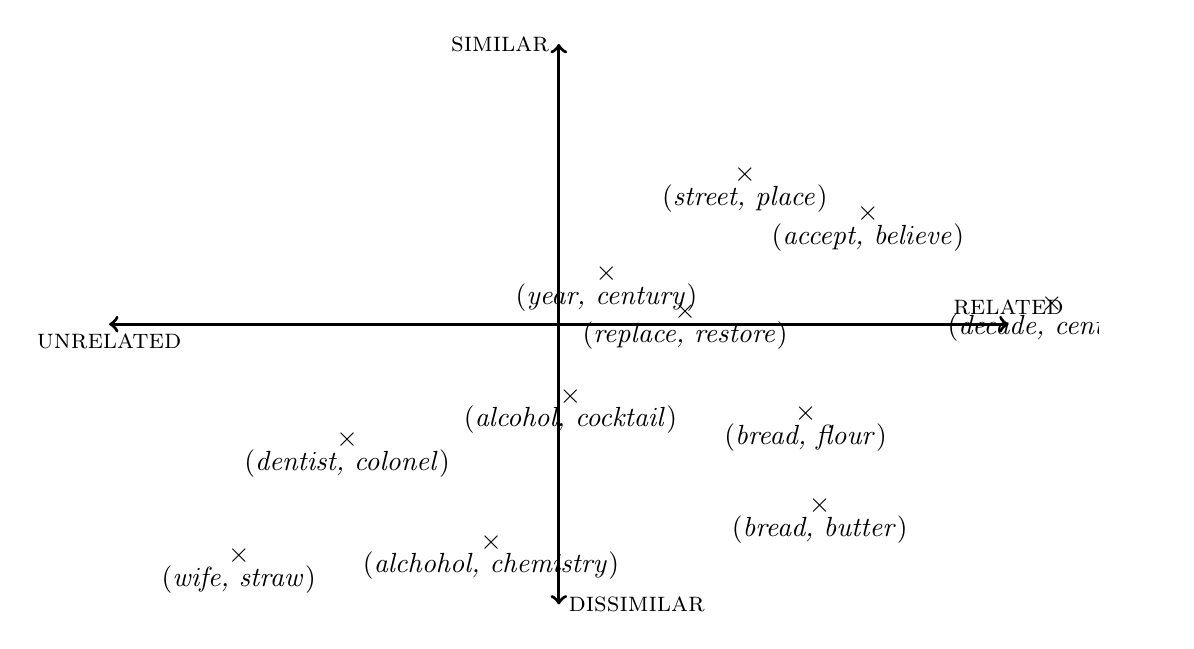
\begin{tikzpicture}
    \begin{axis}[xscale=2,yscale=1.5,hide axis]
      \addplot [<->,very thick] coordinates{(0,5) (10,5)};
      \addplot [<->,very thick] coordinates{(5,0) (5,10)};
      \node at (axis cs: 0,5) [below] {\textsc{unrelated}};
      \node at (axis cs: 10,5) [above] {\textsc{related}};
      \node at (axis cs: 5,0) [right] {\textsc{dissimilar}};
      \node at (axis cs: 5,10) [left] {\textsc{similar}};
      \node at (axis cs: 1.442,0.869) [below] {(\emph{wife, straw})};
      \node at (axis cs: 1.442,0.869) {$\times$};
      \node at (axis cs: 7.901,1.760) [below] {(\emph{bread, butter})};
      \node at (axis cs: 7.901,1.760) {$\times$};
      \node at (axis cs: 2.646,2.940) [below] {(\emph{dentist, colonel})};
      \node at (axis cs: 2.646,2.940) {$\times$};
      \node at (axis cs: 4.247,1.109) [below] {(\emph{alchohol, chemistry})};
      \node at (axis cs: 4.247,1.109) {$\times$};
      \node at (axis cs: 7.744,3.406) [below] {(\emph{bread, flour})};
      \node at (axis cs: 7.744,3.406) {$\times$};
      \node at (axis cs: 5.129,3.714) [below] {(\emph{alcohol, cocktail})};
      \node at (axis cs: 5.129,3.714) {$\times$};
      \node at (axis cs: 6.405,5.218) [below] {(\emph{replace, restore})};
      \node at (axis cs: 6.405,5.218) {$\times$};
      \node at (axis cs: 5.530,5.901) [below] {(\emph{year, century})};
      \node at (axis cs: 5.530,5.901) {$\times$};
      \node at (axis cs: 10.483,5.368) [below] {(\emph{decade, century})};
      \node at (axis cs: 10.483,5.368) {$\times$};
      \node at (axis cs: 8.436,6.970) [below] {(\emph{accept, believe})};
      \node at (axis cs: 8.436,6.970) {$\times$};
      \node at (axis cs: 7.068,7.667) [below] {(\emph{street, place})};
      \node at (axis cs: 7.068,7.667) {$\times$};
    \end{axis}
  \end{tikzpicture}
\caption{Word pair scores along axes of relatedness and similarity as found in 2x2 word co-occurrence window, 400 dimensional, \textsc{indy} type subspaces.}
\label{fig:axes}
\end{figure}

\subsection{Generalising the Models}

\subsection{Frames of Similarity}
\cite{Tversky1977}, in his psychologically motivated reflections on the geometry of similarity, observes that relationships of similarity are fundamentally not symmetric: 

(for comparison, see where the pair (\emph{dentist, colonel}) falls in the space of Figure~\ref{fig:axes}, where it is one of the very few pairs considered to be marginally more similar than related)
